\documentclass{beamer}
\usetheme[progressbar=frametitle]{metropolis}
\setbeamertemplate{frame numbering}[fraction]
\useinnertheme{metropolis}
\useoutertheme{metropolis}
\usefonttheme{metropolis}
\usecolortheme{spruce}

\graphicspath{{./images/}}

\newcommand\boldblue[1]{\textcolor{blue}{\textbf{#1}}}
\newcommand\boldred[1]{\textcolor{red}{\textbf{#1}}}
\newcommand\unfootnote[1]{%
    \begingroup
    \renewcommand\thefootnote{}\footnote{#1}%
    \addtocounter{footnote}{-1}%
    \endgroup
}

\title{Graph Neural Network}
\subtitle{Graph Neural Network Introduction}
\author{}
\institute{}
\date{12 June 2023}

\usepackage{multicol}
\setbeamercovered{transparent=5}

\begin{document}
\metroset{block=fill}
\begin{frame}
\titlepage
    
\end{frame}

\begin{frame}[t]{Why Graphs} \vspace{4pt}
    \begin{itemize}
        \onslide<1->\item Graphs are a general language for describing and analyzing entities with relations/interactions
        \onslide<2->\item Graphs can model many real life complex knowledge / information / data in expressive way
    \end{itemize}
\end{frame}

\begin{frame}[t]{Graph Examples} \vspace{10pt}
    \only<1>{
        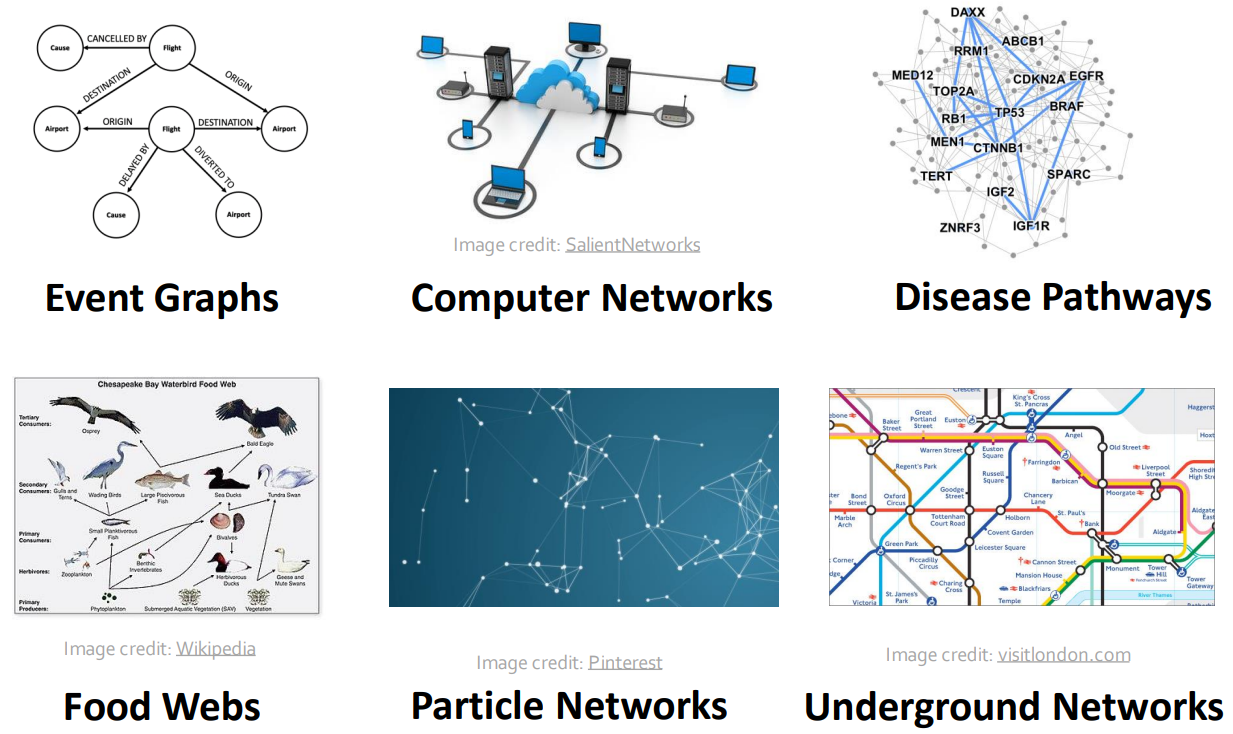
\includegraphics[scale=.35]{graphsOccurances1}
    }
    \only<2>{
        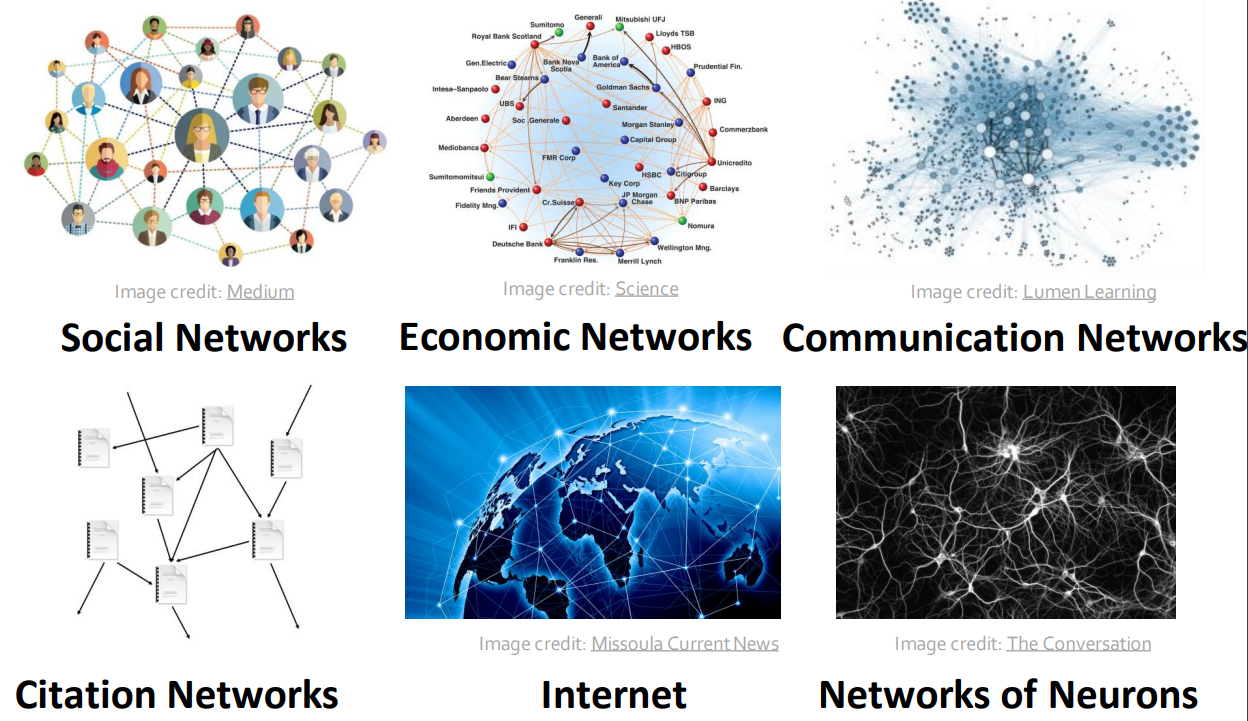
\includegraphics[scale=.33]{graphsOccurances2}
    }
    \only<3>{
        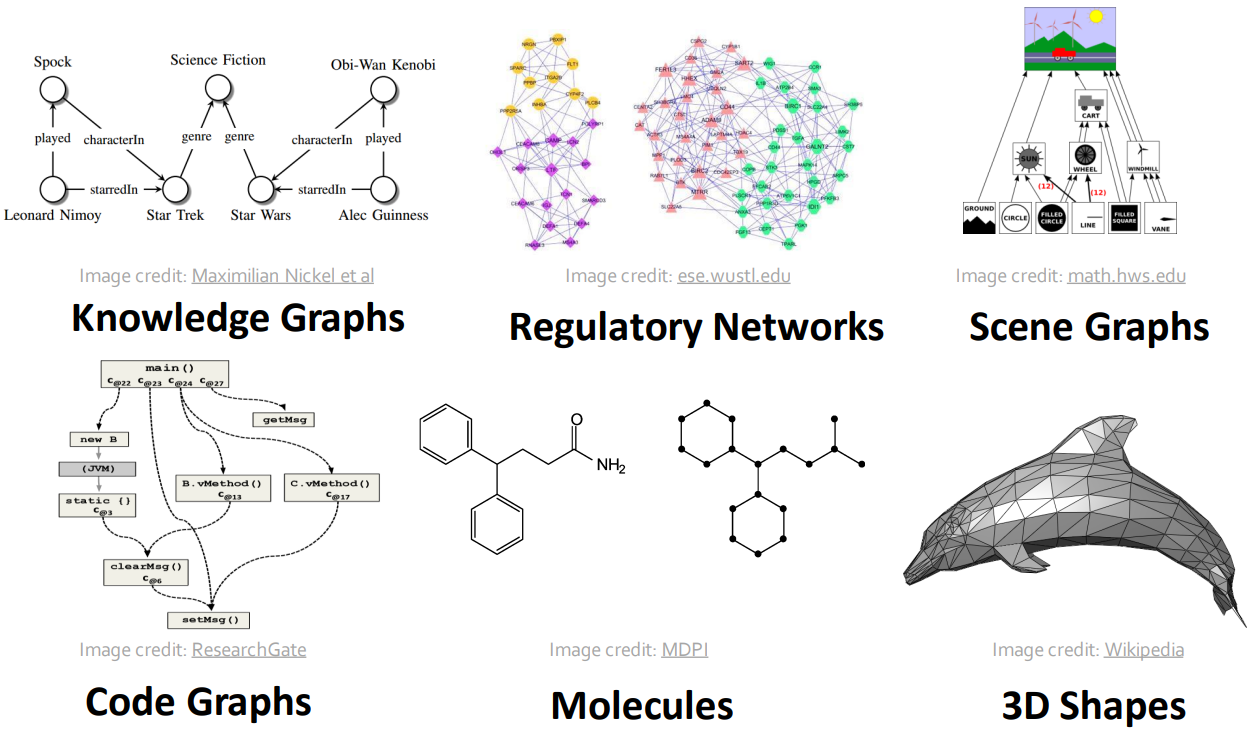
\includegraphics[scale=.35]{graphsOccurances3}
    }
\end{frame}

\begin{frame}[t]{Classic Graph Tasks} \vspace{4pt}
    \only<1>{
        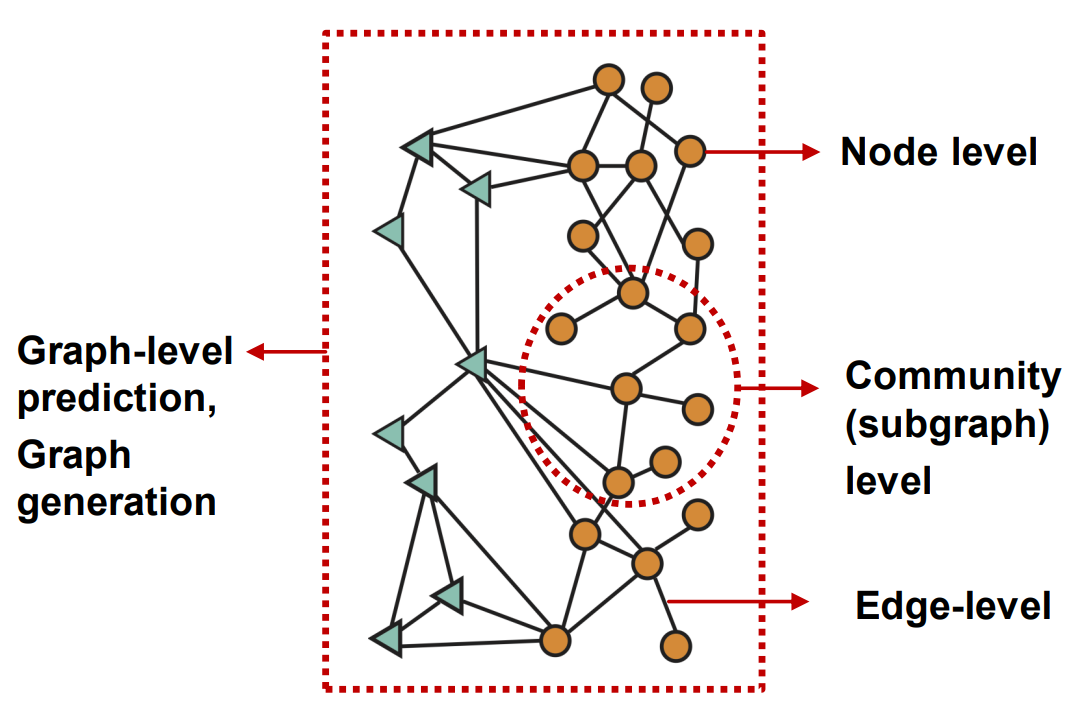
\includegraphics[scale=.35]{classicGraphTasks}
    }
    \only<2>{
        \begin{itemize}
            \item \boldblue{Node classification}: Predict a property of a node\\
                  Example: Categorize online users / items
            \item \boldblue{Link prediction}: Predict whether there are missing links between two nodes\\
                  Example: Knowledge graph completion
            \item \boldblue{Graph classification}: Categorize different graphs\\
                  Example: Molecule property prediction
            \item \boldblue{Clustering}: Detect if nodes form a community\\
                  Example: Social circle detection
            \item \boldblue{Other tasks}:\\
                       Graph generation: Drug discovery\\
                       Graph evolution: Physical simulation
        \end{itemize}
    }
\end{frame}

\begin{frame}[t]{Why is Graph Deep Learning Hard} \vspace{4pt}
    \begin{block}{Networks are complex}
        \begin{itemize}
            \item Arbitrary size and complex topological structure (i.e., no spatial locality like grids)
            \item No fixed node ordering or reference point
            \item Often dynamic and have multimodal features
        \end{itemize}
    \end{block}

    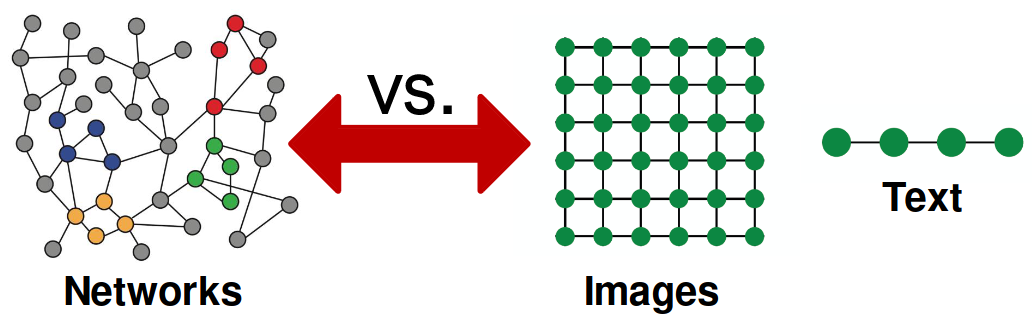
\includegraphics[scale=.3]{networkVsImageAndText}
\end{frame}

\begin{frame}[t]{Traditional Approaches} \vspace{4pt}

    \only<1->{
        \boldblue{Traditional approaches are feature engineering based:}

        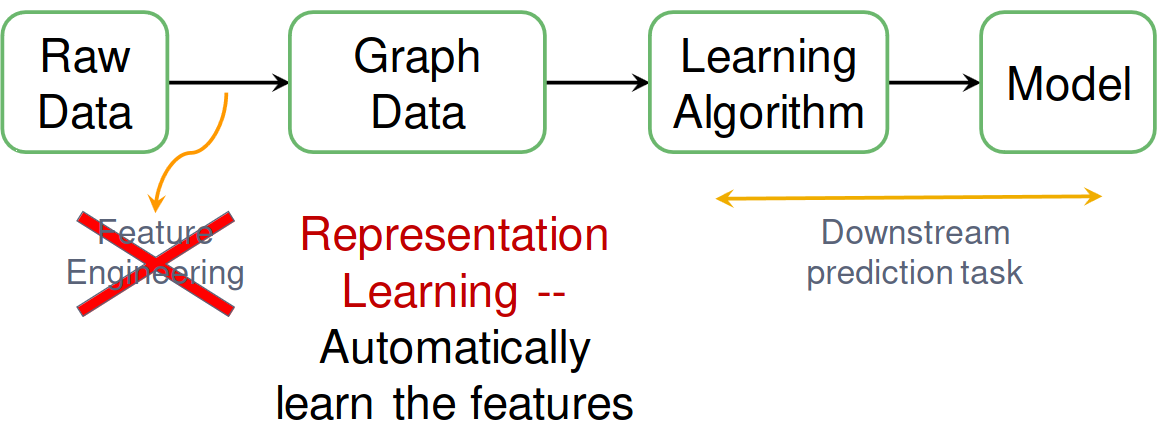
\includegraphics[scale=.27]{traditionalApproaches}
    }
    \only<2>{
        \begin{block}{Feature Extraction}
            Node level, link level, graph level statistical deterministic feature are extracted.
        \end{block}
    }

\end{frame}


\section{Graph Neural Network Based Approaches}

\begin{frame}[t]{Node Embedding}\vspace{10pt}
    Each node can be identified with a vector.\vspace{20pt}
    
    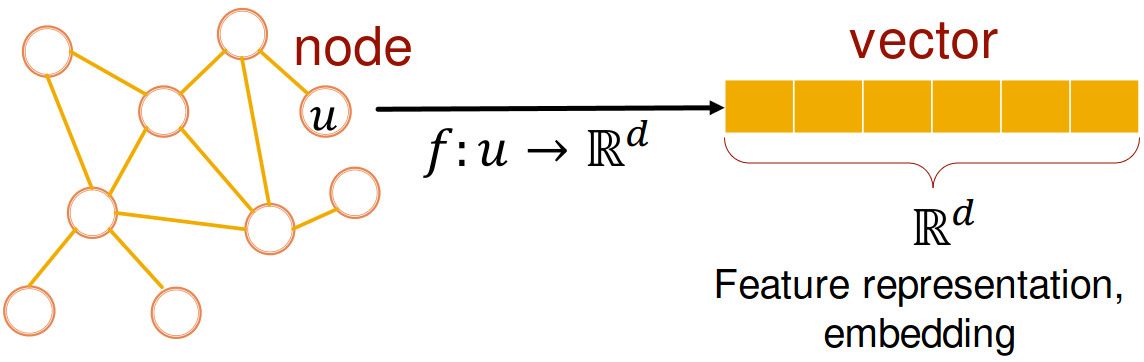
\includegraphics[scale=.26]{nodeEmbeddingGoal}
\end{frame}

\begin{frame}[t]{Embedding Goals}

    \begin{block}{Task: Map nodes into an embedding space}
    
        \begin{itemize}
        
            \item Similarity of embeddings between nodes indicates their similarity in the network. For example: Both nodes are close to each other (connected by an edge)

            \item Encode network information
            
            \item Potentially used for many downstream predictions
        \end{itemize}
        
    \end{block}

    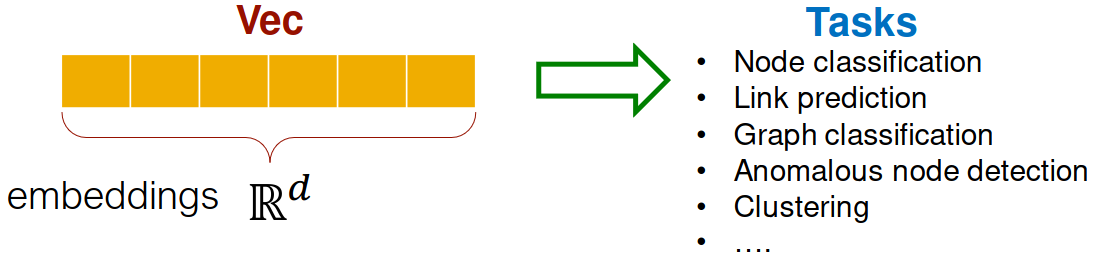
\includegraphics[scale=.33]{nodeEmbeddingTasks}
    
\end{frame}

\begin{frame}[t]{Example Node Embedding}
    2D embedding of nodes of the Zachary’s Karate Club network:\\ \vspace{20pt}
    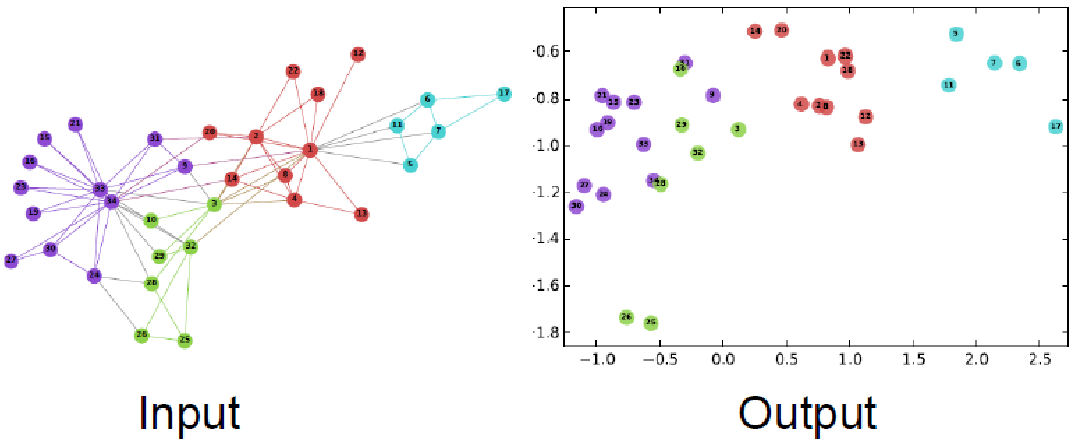
\includegraphics[scale=.3]{images/Zakarys2DExample.png}
\end{frame}

\begin{frame}[t]{Word2Vec}
    \only<1>{
        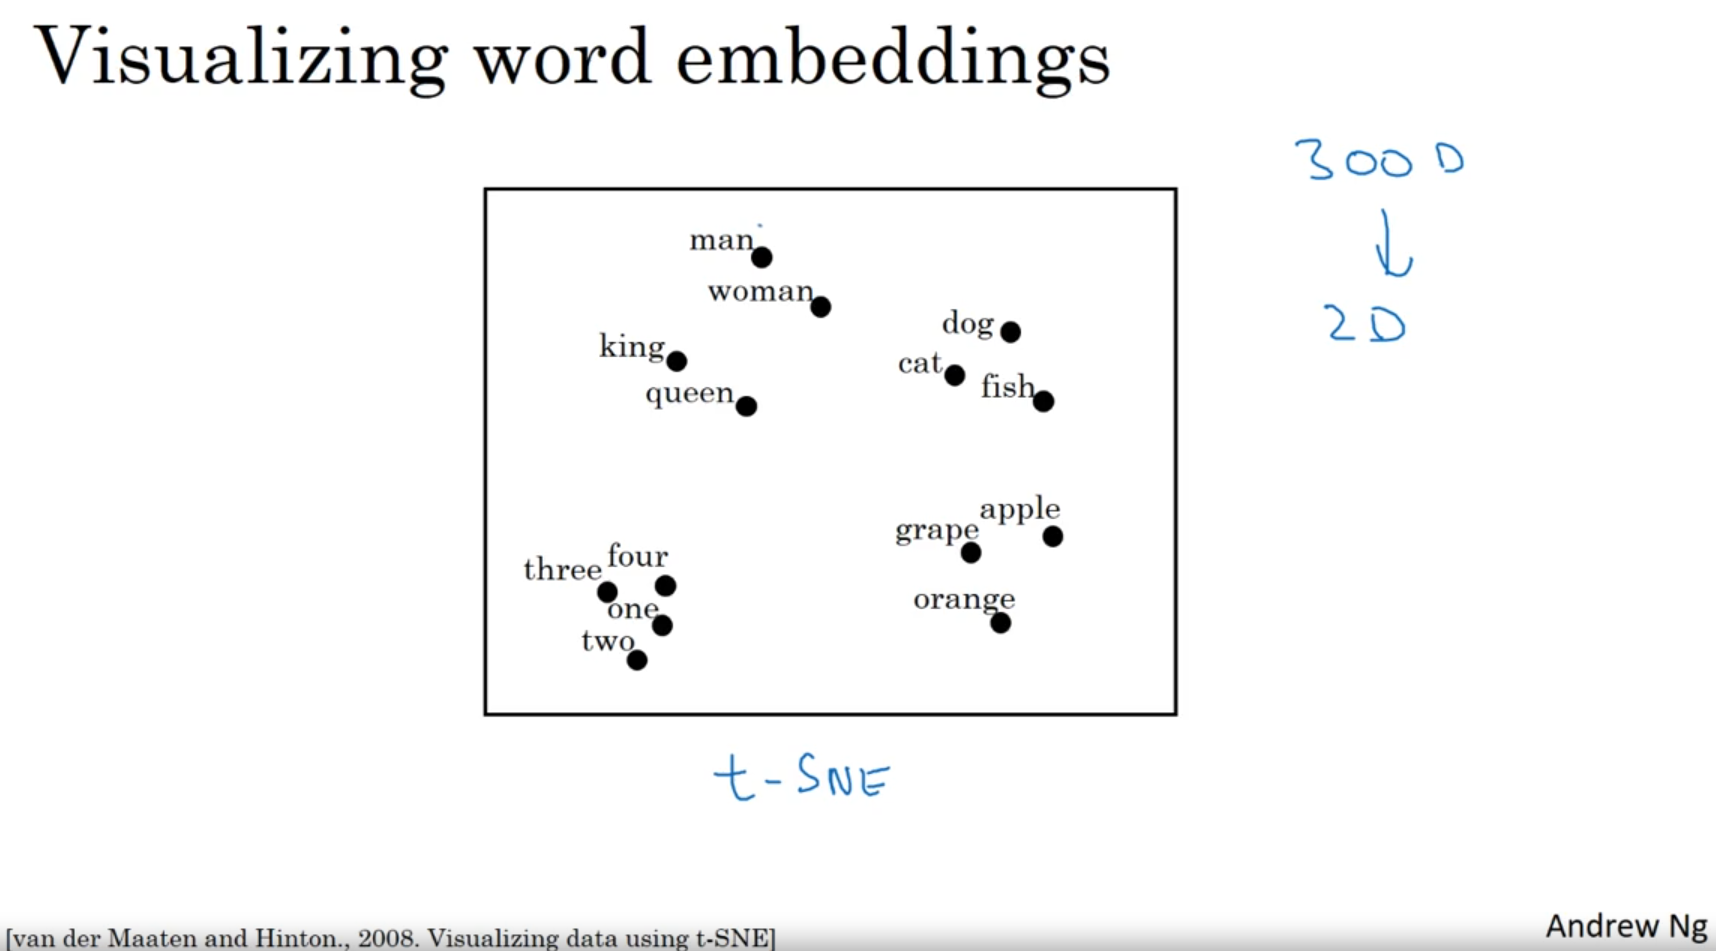
\includegraphics[scale=.18]{images/VisualizeWordEmbeddingWord2Vec.png}
        \unfootnote{
            \href{https://towardsdatascience.com/nlp-101-word2vec-skip-gram-and-cbow-93512ee24314}{NLP 101: Word2Vec — Skip-gram and CBOW}\\
            \href{http://cs224d.stanford.edu/lecture_notes/notes1.pdf}{Lecture notes CS224D: Deep Learning for NLP Part-I}\\
            \href{https://www.coursera.org/learn/nlp-sequence-models/home/week/2}{Coursera - Andrew Ng - Sequence Model - Week 2}
        }
    }
    \only<2>{
        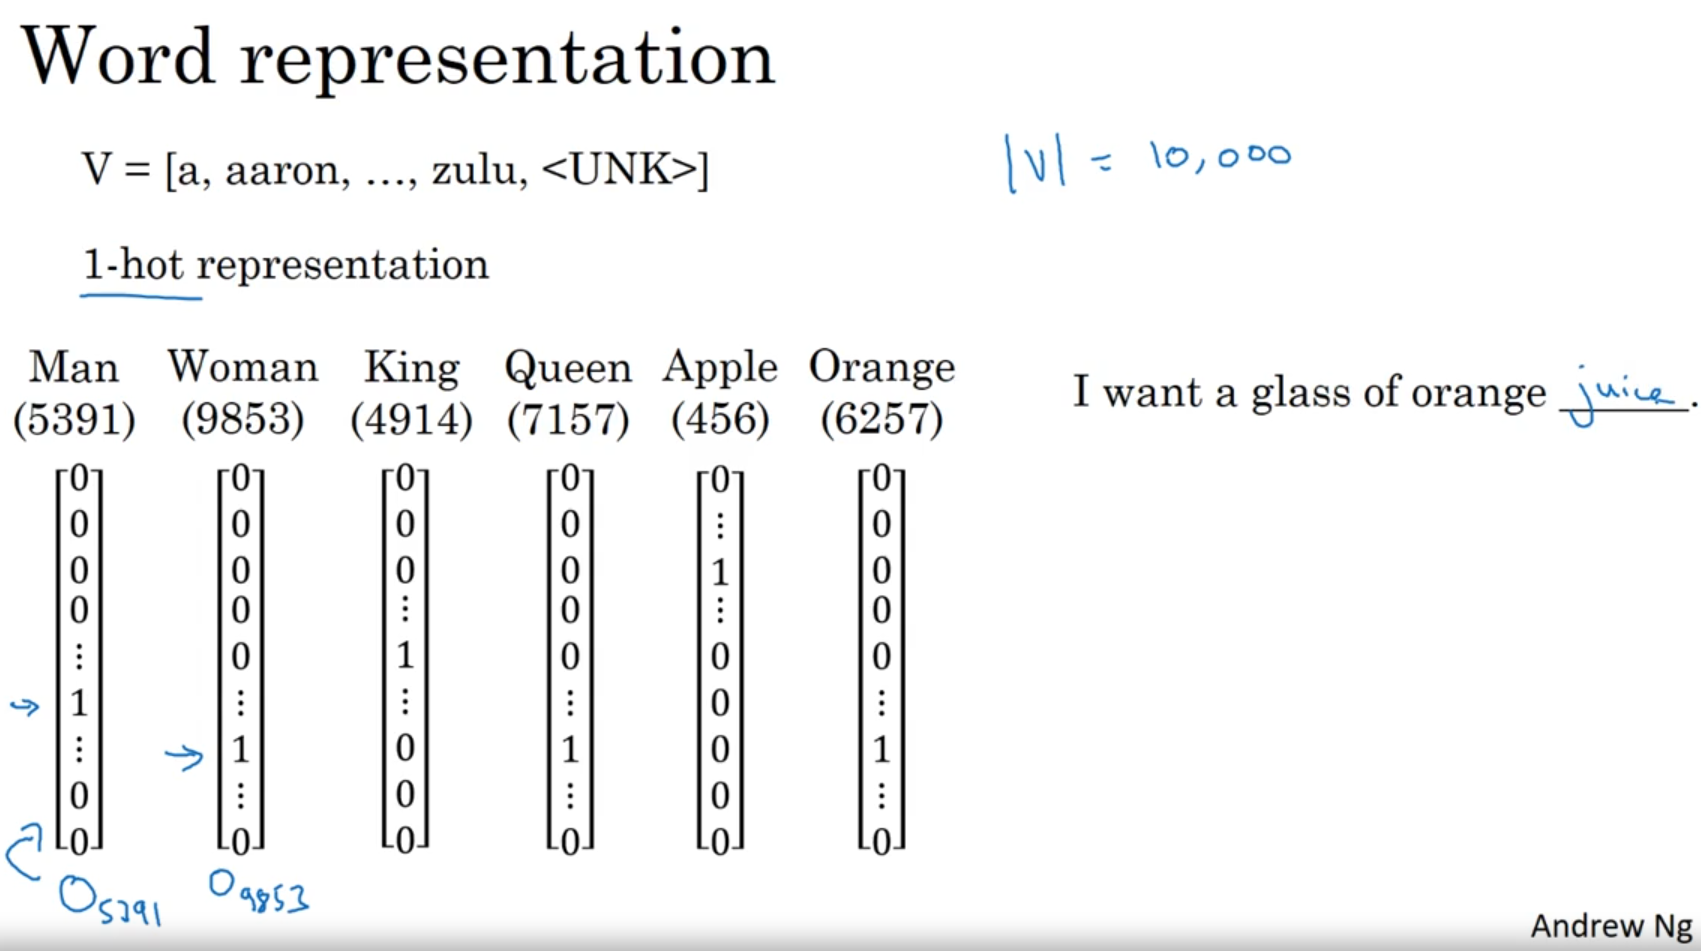
\includegraphics[scale=.18]{images/WordRepresentationOfWord2Vec.png}
    }
    \only<3>{
        \begin{block}{CBOW Objective}
            We want to predict the target from the context.
        \end{block}
        The \boldblue{brown fox} \boldred{jumped} \boldblue{over the} lazy dog.
        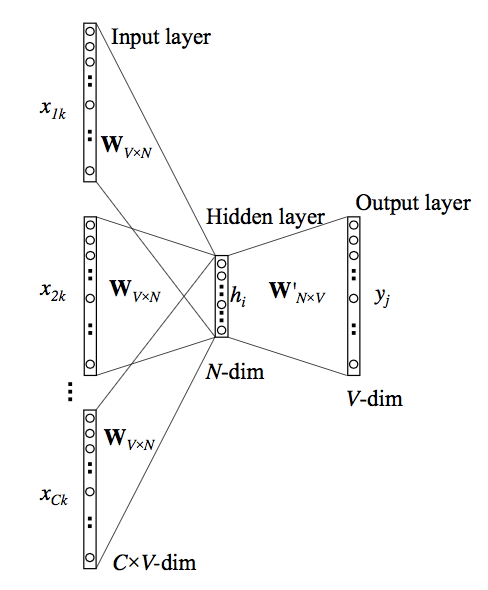
\includegraphics[scale=.29]{CBOWWord2Vec}

    }
\end{frame}

\begin{frame}[t]{DeepWalk}
    \unfootnote{
        \href{https://towardsdatascience.com/deepwalk-its-behavior-and-how-to-implement-it-b5aac0290a15}{DeepWalk: Its Behavior and How to Implement It}
    }

    \begin{itemize}
        \item For each node, perform N “random steps” starting from that node
        \item Treat each walk as a sequence of node-id strings
        \item Given a list of these sequences, train a word2vec model using the Skip-Gram algorithm on these string sequences
    \end{itemize}

    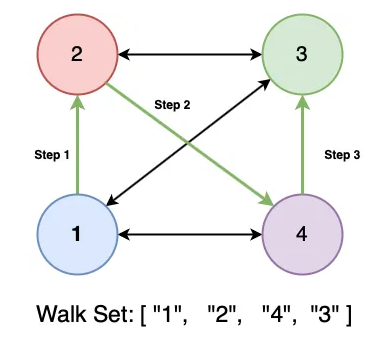
\includegraphics[scale=.33]{images/DeepWalkRandomWalk.png}
\end{frame}

\begin{frame}[t]{Node2Vec}
    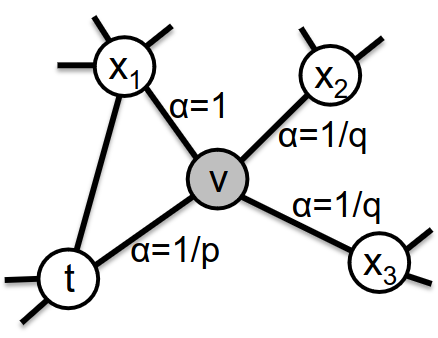
\includegraphics[scale=.35]{Node2VecExploration}

    \boldblue{Biased random walk to explore more like DFS or BFS}
\end{frame}
\begin{frame}[t]{Graph Convolutional Network}
    \begin{block}{GCN Setup}
        \begin{itemize}
            \item an input feature matrix $N\times F^0$ feature matrix, $X$, where $N$ is the number of nodes and $F^0$ is the number of input features for each node
            \item an $N\times N$ matrix representation of the graph structure such as the adjacency matrix $A$ of $G$
        \end{itemize}
    \end{block}

    $$ H^i = f(H^{i-1}, A) $$
    $$ = \sigma(AH^{i-1}W)$$

    \begin{block}{Simplification}
        $$ H = AX $$
    \end{block}
\end{frame}

\begin{frame}[t]{Graph Convolutional Network}
    \begin{columns}[onlytextwidth]
        
        \column{.4\textwidth}
        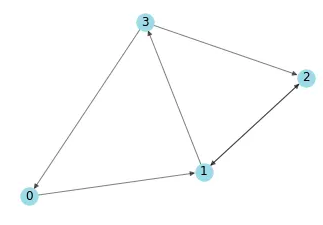
\includegraphics[scale=.38]{images/GCNExampleNet.png}
                                               \column{.6\textwidth}
                                               \begin{math}
                                                    A =
                                                        \begin{bmatrix}
                                                            0 & 1 & 0 & 0\\
                                                            0 & 0 & 1 & 1\\
                                                            0 & 1 & 0 & 0\\
                                                            1 & 0 & 1 & 0
                                                        \end{bmatrix}
                                                    X = \begin{bmatrix}
                                                            0 &  0\\
                                                            1 & -1\\
                                                            2 & -2\\
                                                            3 & -3
                                                        \end{bmatrix}
                                                \end{math}
    \end{columns}

    \begin{block}{Issues}
        \begin{itemize}
            \item Add self loop
            \item Normalize
        \end{itemize}
    \end{block}

    Finally: $f(X, A) = D^{-1} \hat{A} X W$

    \unfootnote{
        \href{https://towardsdatascience.com/how-to-do-deep-learning-on-graphs-with-graph-convolutional-networks-7d2250723780}{How to do Deep Learning on Graphs with Graph Convolutional Networks}
    }
    
\end{frame}

\begin{frame}[t]{GraphSAGE}
    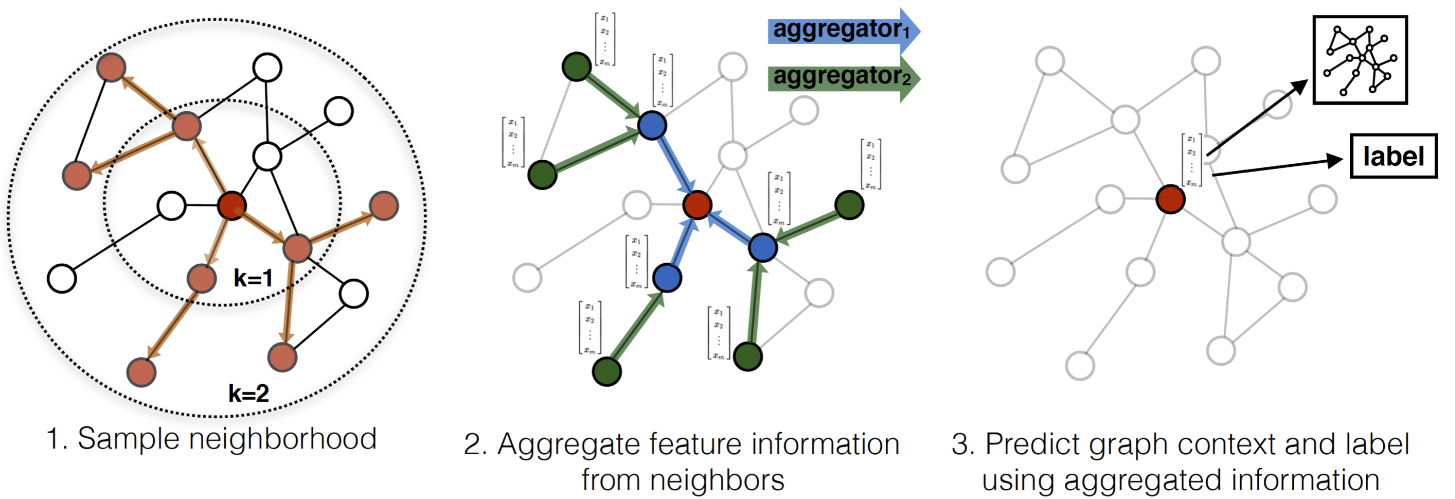
\includegraphics[scale=.2]{GraphSAGE}
    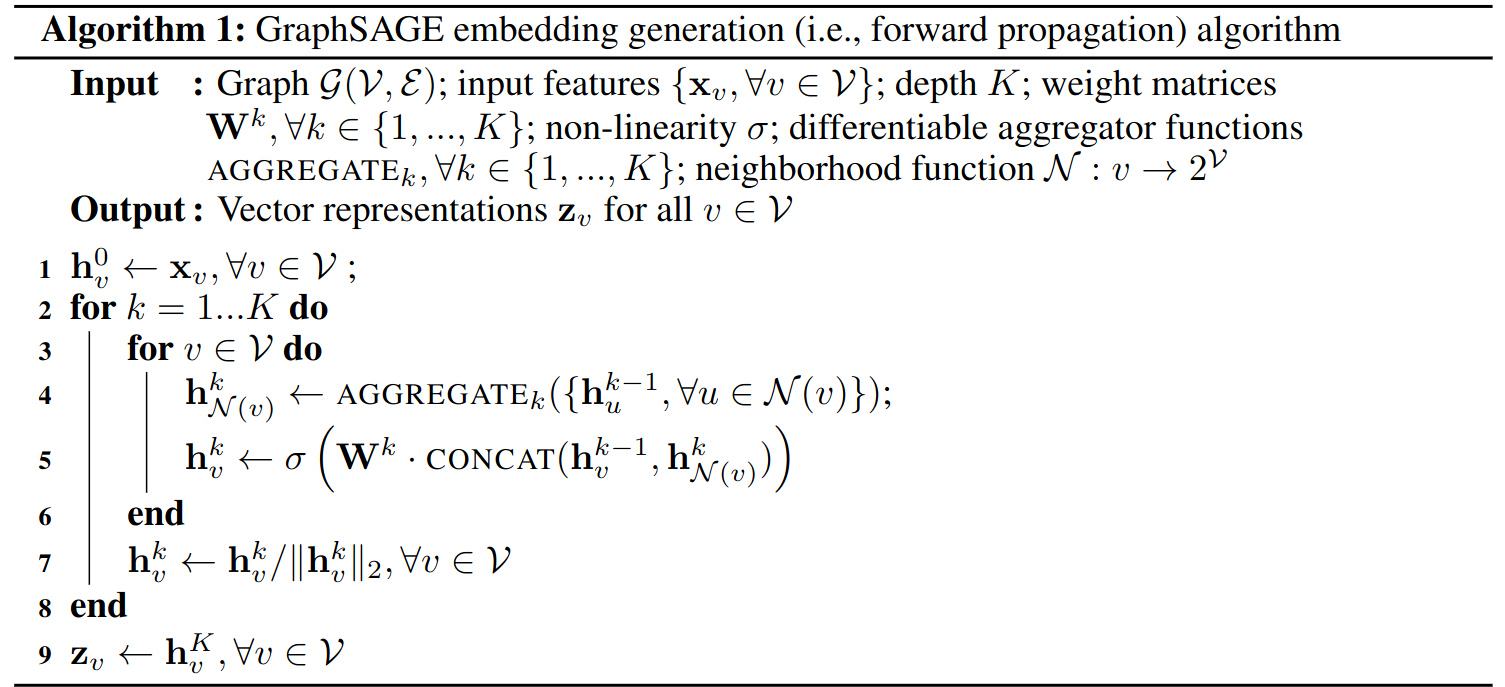
\includegraphics[scale=.18]{GraphSAGEAlgo}
\end{frame}

\begin{frame}[t]{GraphSAGE Loss}
    Encourages nearby nodes to have similar representations, while enforcing
    that the representations of disparate nodes are highly distinct

    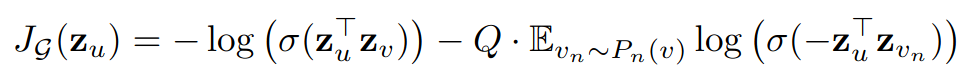
\includegraphics[scale=.27]{GraphSAGELoss}
\end{frame}

\begin{frame}[standout]
\flushleft
Questions?
\end{frame}
\end{document}